\documentclass[12pt]{article}
\usepackage[utf8]{inputenc}
\usepackage[T1]{fontenc}
\usepackage[spanish,es-nodecimaldot]{babel}
\usepackage{amsmath}
\usepackage{amssymb}
\usepackage{physics}
\usepackage{siunitx}
\usepackage{geometry}
\usepackage{graphicx}
\usepackage{float}
\usepackage{array}
\usepackage{booktabs}
\usepackage{tikz}
\usetikzlibrary{babel,arrows.meta,positioning}
\usepackage{xcolor}
\usepackage{hyperref}
\geometry{margin=2.5cm}

\definecolor{unapBlue}{RGB}{0,63,122}
\definecolor{unapGold}{RGB}{174,126,37}

\sisetup{
  input-decimal-markers = {.,},
  output-decimal-marker = {.},
  group-separator = {\,},
  per-mode = symbol
}

\hypersetup{
  colorlinks=true,
  linkcolor=blue!45!black,
  urlcolor=blue!45!black,
  pdftitle={Resolución Completa de Examen de Turbomáquinas}
}

\newcommand{\figuraFaltante}{\emph{La figura no fue proporcionada; por tanto, no es posible fijar una letra o sentido absoluto sin ambigüedad. Se resuelve mediante el criterio físico correspondiente.}}
\newcommand{\resultado}[1]{\[
  \boxed{\displaystyle #1}
\]}

\begin{document}

\pagenumbering{gobble}
\newgeometry{top=1.25cm,bottom=1.35cm,left=1.8cm,right=1.8cm}
\begin{titlepage}
\thispagestyle{empty}
\centering

\noindent
\begin{minipage}[c]{0.18\textwidth}
  \centering
  
\includegraphics[height=2.35cm,keepaspectratio]{../imagenes/logo_unap.png}
\end{minipage}%
\begin{minipage}[c]{0.64\textwidth}
  \centering
  {\large\bfseries\color{unapBlue} UNIVERSIDAD NACIONAL DEL ALTIPLANO DE PUNO\par}
  \vspace{0.12cm}
  {\small\bfseries FACULTAD DE INGENIERÍA MECÁNICA ELÉCTRICA, ELECTRÓNICA Y SISTEMAS\par}
  \vspace{0.10cm}
  {\small\bfseries ESCUELA PROFESIONAL DE INGENIERÍA MECÁNICA ELÉCTRICA\par}
\end{minipage}%
\begin{minipage}[c]{0.18\textwidth}
  \centering
  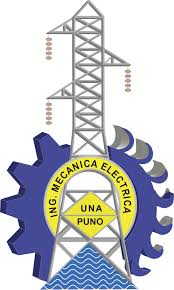
\includegraphics[height=2.35cm,keepaspectratio]{../imagenes/logo_mecanica.png}
\end{minipage}

\vspace{0.30cm}
{\color{unapGold}\rule{\textwidth}{1.3pt}}

\vspace{0.35cm}
{\large\bfseries\color{unapBlue} SOLUCIONARIO ACADÉMICO\par}
\vspace{0.28cm}

\setlength{\fboxrule}{0.9pt}
\setlength{\fboxsep}{10pt}
\fcolorbox{unapBlue}{unapBlue!4}{%
  \begin{minipage}{0.88\textwidth}
    \centering
    {\LARGE\bfseries Resolución Completa de Examen\par}
    \vspace{0.12cm}
    {\LARGE\bfseries de Turbomáquinas\par}
  \end{minipage}%
}

\vspace{0.30cm}

% Símbolo técnico central: rodete radial y triángulo de velocidades.
\begin{tikzpicture}[>=Latex,scale=0.67]
  \draw[line width=1.0pt,fill=unapBlue!4] (0,0) circle (2.25);
  \draw[line width=1.0pt,fill=white] (0,0) circle (0.68);
  \foreach \a in {0,45,...,315}{
    \draw[line width=1.5pt,unapBlue]
      (\a:2.20) .. controls ({\a+10}:1.78) and ({\a+24}:1.10) .. ({\a+31}:0.70);
  }
  \draw[-{Latex[length=3mm]},line width=1.3pt,unapGold] (0,2.65) arc (90:165:2.65);
  \node[unapGold,font=\small\bfseries] at (-2.55,2.25) {rotación};
  \draw[-{Latex[length=3mm]},line width=1.2pt,red!70!black]
    (3.2,0.95)--(2.10,0.65) node[midway,above] {flujo};
  \node[unapBlue,font=\bfseries] at (0,-2.70) {RODETE CENTRÍFUGO};
\end{tikzpicture}

\vspace{0.15cm}

\begin{tabular}{@{}>{\bfseries\color{unapBlue}}r@{\hspace{0.55cm}}l@{}}
Asignatura: & Turbomáquinas \\
Documento: & Resolución completa de examen \\
Responsable: & CRUZ CABRERA ARMANDO TITO \\
Sección: & GRUPO A \\
Especialidad: & Ingeniería Mecánica Eléctrica \\
\end{tabular}

\vspace{0.30cm}

\setlength{\fboxrule}{0.7pt}
\setlength{\fboxsep}{8pt}
\fcolorbox{unapGold}{white}{%
  \begin{minipage}{0.88\textwidth}
    \centering
    {\bfseries\color{unapBlue} INTEGRANTES\par}
    \vspace{0.15cm}
    \renewcommand{\arraystretch}{1.18}
    \begin{tabular}{@{}c@{\hspace{0.65cm}}l@{}}
      \toprule
      \textbf{Código} & \textbf{Apellidos y nombres} \\
      \midrule
      227417 & CCALLA QUISPE CARLOS MARTIN \\
      228468 & SIGUAYRO COILA DILMAR HUMBERTO \\
      227420 & RIVERA QUISPE ABEL YOVANI \\
      228447 & MAMANI GALINDO RENZO GABRIEL \\
      227368 & AQUILES TAYLOR RAMOS YAPO \\
      \bottomrule
    \end{tabular}
  \end{minipage}%
}

\vfill
{\color{unapGold}\rule{0.42\textwidth}{0.9pt}}\par
\vspace{0.12cm}
{\large\bfseries Puno, Perú\par}
{\large\bfseries 2026\par}
\end{titlepage}
\restoregeometry

\pagenumbering{roman}
\tableofcontents
\newpage
\pagenumbering{arabic}

\section*{Introducción}
\addcontentsline{toc}{section}{Introducción}
El presente documento desarrolla, en el orden propuesto, los problemas del examen de
Turbomáquinas. Se emplean balances de energía, ecuaciones de Euler, triángulos de
velocidades, relaciones de semejanza y principios de mecánica de fluidos. Todas las
sustituciones numéricas se efectúan en el Sistema Internacional (SI). Cuando el enunciado
depende de una figura ausente, se conserva la solución en forma paramétrica o se establece
el criterio físico que permitiría resolverla al disponer del dibujo original.

\section*{Hipótesis generales}
\addcontentsline{toc}{section}{Hipótesis generales}
Salvo indicación contraria, se considera flujo estacionario, agua incompresible con
$\rho=\SI{1000}{kg.m^{-3}}$, aceleración de la gravedad $g=\SI{9.81}{m.s^{-2}}$ y
velocidades medias uniformes en las secciones. En los análisis ideales de rodetes se
desprecian pérdidas mecánicas, volumétricas e hidráulicas, excepto cuando se introduce
explícitamente una eficiencia o un coeficiente de resbalamiento. Los ángulos se interpretan
desde la tangente cuando así se indica; si la figura ausente impide confirmar la convención,
se declara la ambigüedad.

\section{Primera Parte}

\subsection{Problema 1}

\subsubsection*{Enunciado}
Determinar la altura efectiva y la potencia del motor de una bomba centrífuga que transporta
$\SI{100}{L.s^{-1}}$ entre dos reservorios. La succión mide $\SI{6}{m}$ y la descarga
$\SI{150}{m}$; ambas tuberías tienen diámetro $\SI{250}{mm}$.

\figuraFaltante En particular, falta el desnivel geométrico $z_d-z_s$ de la figura 1.

\subsubsection*{Datos}
\[
Q=\SI{100}{L.s^{-1}}=\SI{0.100}{m^3.s^{-1}},\quad
D=\SI{0.250}{m},\quad L_s=\SI{6}{m},\quad L_d=\SI{150}{m}.
\]
Se definen $L_T=L_s+L_d=\SI{156}{m}$, $f$ como factor de Darcy,
$K_{\mathrm{tot}}$ como suma de coeficientes de pérdidas locales y $\eta$ como eficiencia
global bomba--motor.

\subsubsection*{Fundamento teórico}
Entre las superficies libres de dos reservorios, la ecuación de Bernoulli extendida incluye
la energía añadida por la bomba y las pérdidas de carga. Como ambas superficies están a
presión atmosférica y sus velocidades son despreciables,
\[
H_B=(z_d-z_s)+h_L.
\]
Las pérdidas distribuidas se calculan con Darcy--Weisbach y las locales con
$h_m=K_{\mathrm{tot}}V^2/(2g)$.

\subsubsection*{Hipótesis y simplificaciones}
Flujo permanente e incompresible; diámetro constante; velocidad despreciable en las
superficies libres; presión atmosférica en ambos reservorios. No se asignan valores a
$z_d-z_s$, $f$, $K_{\mathrm{tot}}$ ni $\eta$ porque no aparecen en el material suministrado.

\subsubsection*{Desarrollo}
El área y la velocidad media son
\[
A=\frac{\pi D^2}{4},\qquad V=\frac{Q}{A}.
\]
La pérdida total es
\[
h_L=f\frac{L_T}{D}\frac{V^2}{2g}
   +K_{\mathrm{tot}}\frac{V^2}{2g}.
\]
La potencia hidráulica comunicada al agua y la potencia requerida por el motor son
\[
P_h=\rho gQH_B,\qquad P_{\mathrm{motor}}=\frac{P_h}{\eta}.
\]

\subsubsection*{Cálculos}
\begin{align*}
A&=\frac{\pi(\SI{0.250}{m})^2}{4}=\SI{0.049087}{m^2},\\
V&=\frac{\SI{0.100}{m^3.s^{-1}}}{\SI{0.049087}{m^2}}
  =\SI{2.037}{m.s^{-1}},\\
\frac{V^2}{2g}&=\frac{(\SI{2.037}{m.s^{-1}})^2}
 {2(\SI{9.81}{m.s^{-2}})}=\SI{0.2115}{m},\\
f\frac{L_T}{D}\frac{V^2}{2g}
&=f\frac{\SI{156}{m}}{\SI{0.250}{m}}(\SI{0.2115}{m})
=131.99f\ \si{m}.
\end{align*}
Por tanto,
\[
H_B=(z_d-z_s)+131.99f+0.2115K_{\mathrm{tot}}\quad [\si{m}].
\]
Además,
\begin{align*}
P_h&=(\SI{1000}{kg.m^{-3}})(\SI{9.81}{m.s^{-2}})
(\SI{0.100}{m^3.s^{-1}})H_B\\
&=981H_B\ \si{W}=0.981H_B\ \si{kW}.
\end{align*}

\subsubsection*{Resultado}
\resultado{H_B=(z_d-z_s)+131.99f+0.2115K_{\mathrm{tot}}\ \si{m}}
\resultado{P_{\mathrm{motor}}=\frac{0.981}{\eta}
\left[(z_d-z_s)+131.99f+0.2115K_{\mathrm{tot}}\right]\ \si{kW}}

\subsubsection*{Discusión}
La dimensión de cada término de $H_B$ es longitud. Asimismo,
\[
[\rho gQH]
=\si{kg.m^{-3}}\,\si{m.s^{-2}}\,\si{m^3.s^{-1}}\,\si{m}
=\si{kg.m^2.s^{-3}}=\si{W}.
\]
Sin la figura 1 y sin los coeficientes hidráulicos y la
eficiencia no existe un único resultado numérico.

\subsection{Problema 2}

\subsubsection*{Enunciado}
Una bomba centrífuga tiene rotor de doble succión y número específico de caudal global
$N_q=14.1$. Determinar el $N_q$ de diseño.

\subsubsection*{Datos}
\[
N_{q,\mathrm{global}}=14.1,\qquad Q_{\mathrm{ojo}}=\frac{Q_{\mathrm{total}}}{2}.
\]

\subsubsection*{Fundamento teórico}
El número específico de caudal se define por
\[
N_q=\frac{n\sqrt{Q}}{H^{3/4}}.
\]
En doble succión, los dos ojos trabajan a la misma velocidad de giro y desarrollan la misma
altura, pero cada uno procesa la mitad del caudal total.

\subsubsection*{Hipótesis y simplificaciones}
El reparto de caudal es simétrico y no hay desbalance entre los dos lados del rodete.

\subsubsection*{Desarrollo}
Para un ojo,
\[
N_{q,\text{diseño}}
=\frac{n\sqrt{Q_{\mathrm{total}}/2}}{H^{3/4}}
=\frac{1}{\sqrt{2}}\frac{n\sqrt{Q_{\mathrm{total}}}}{H^{3/4}}
=\frac{N_{q,\mathrm{global}}}{\sqrt{2}}.
\]

\subsubsection*{Cálculos}
\[
N_{q,\text{diseño}}=\frac{14.1}{\sqrt{2}}=9.970.
\]

\subsubsection*{Resultado}
\resultado{N_{q,\text{diseño}}=9.97\approx 10.0}

\subsubsection*{Discusión}
El valor disminuye por $\sqrt{2}$, no por 2, porque el caudal aparece bajo raíz cuadrada en
la definición de $N_q$.

\subsection{Problema 3}

\subsubsection*{Enunciado}
Trazar los álabes del estator asociado a un rotor mostrado en la figura 3.

\figuraFaltante

\subsubsection*{Datos}
No se proporcionan geometría, velocidades ni ángulos. Se dispone únicamente de la relación
vectorial fundamental
\[
\vb C=\vb U+\vb W.
\]

\subsubsection*{Fundamento teórico}
La velocidad absoluta $\vb C$ es observada desde la carcasa; $\vb U$ es la velocidad
periférica del rotor, y $\vb W$ es la velocidad relativa observada desde el álabe. Para una
entrada sin choque, $\vb W_1$ debe ser tangente a la línea media del álabe móvil.

\subsubsection*{Hipótesis y simplificaciones}
Se supone diseño ideal sin incidencia a la entrada del rotor y estator de espesor despreciable
en el esquema conceptual.

\subsubsection*{Desarrollo}
Conocidos el sentido de $\vb U_1$ y la tangente del álabe móvil, se fija $\vb W_1$. El cierre
del triángulo $\vb C_1=\vb U_1+\vb W_1$ determina la dirección de salida del estator. Por
consiguiente, la línea media de cada álabe fijo debe ser tangente a $\vb C_1$ en su borde de
salida.

\subsubsection*{Cálculos}
No hay cálculo numérico posible. El trazado vectorial conceptual es:
\begin{figure}[H]
\centering
\begin{tikzpicture}[>=Latex,font=\small]
  % Geometría conceptual del paso estator--rotor
  \begin{scope}[shift={(-4.3,0)}]
    \node[font=\bfseries] at (1.8,2.65) {Orientación de los álabes};
    \draw[very thick,red!70!black]
      (0.1,-1.25) .. controls (0.55,-0.25) and (1.15,0.65) .. (1.85,1.55);
    \draw[very thick,red!70!black]
      (0.85,-1.25) .. controls (1.30,-0.25) and (1.90,0.65) .. (2.60,1.55);
    \draw[very thick,blue!70!black]
      (3.10,-1.20) .. controls (2.85,-0.25) and (2.42,0.72) .. (1.85,1.55);
    \draw[very thick,blue!70!black]
      (3.85,-1.20) .. controls (3.60,-0.25) and (3.17,0.72) .. (2.60,1.55);
    \draw[-{Latex[length=3mm]},line width=1.2pt,red!70!black]
      (0.85,-0.75)--(2.15,1.05) node[midway,left=2pt,fill=white,inner sep=1pt] {$\vb C_1$};
    \draw[-{Latex[length=3mm]},line width=1.2pt,blue!70!black]
      (3.40,-0.80)--(2.15,1.05) node[midway,right=2pt,fill=white,inner sep=1pt] {$\vb W_1$};
    \node[red!70!black] at (0.85,-1.55) {álabes fijos};
    \node[blue!70!black] at (3.35,-1.55) {álabes móviles};
    \node[align=center] at (2.05,-2.25) {Tangencia en ambos bordes:\\salida fija y entrada móvil};
  \end{scope}

  % Triángulo de velocidades separado para evitar superposiciones
  \begin{scope}[shift={(2.0,-0.15)}]
    \node[font=\bfseries] at (1.55,2.80) {Triángulo de entrada};
    \coordinate (O) at (0,0);
    \coordinate (A) at (3.3,0);
    \coordinate (B) at (1.15,2.10);
    \draw[-{Latex[length=3mm]},line width=1.2pt] (O)--(A)
      node[midway,below=5pt] {$\vb U_1$};
    \draw[-{Latex[length=3mm]},line width=1.2pt,blue!70!black] (A)--(B)
      node[midway,right=5pt,fill=white,inner sep=1pt] {$\vb W_1$};
    \draw[-{Latex[length=3mm]},line width=1.2pt,red!70!black] (O)--(B)
      node[midway,left=5pt,fill=white,inner sep=1pt] {$\vb C_1$};
    \draw[dashed,gray] (B)--(1.15,0);
    \node[align=center] at (1.65,-0.72)
      {$\vb C_1=\vb U_1+\vb W_1$};
  \end{scope}
\end{tikzpicture}
\caption{Criterio de orientación del estator para entrada sin choque.}
\end{figure}

\subsubsection*{Resultado}
\resultado{\text{El borde de salida del estator debe ser tangente a }\vb C_1
\text{ y }\vb W_1\text{ debe ser tangente al rotor.}}

\subsubsection*{Discusión}
Sin la figura no puede reproducirse la curvatura exacta ni asignarse una orientación absoluta;
el criterio de tangencia sí es único y físicamente suficiente para completar el dibujo original.

\subsection{Problema 4}

\subsubsection*{Enunciado}
Dibujar el rotor de una turbina Francis con $\beta_2=90^\circ$, $\beta_1=30^\circ$,
$\alpha_1=90^\circ$, giro antihorario y directrices a $20^\circ$, incluyendo triángulos de
velocidad de entrada y salida.

\subsubsection*{Datos}
\[
\beta_1=30^\circ,\qquad \beta_2=90^\circ,\qquad \alpha_1=90^\circ,
\qquad \theta_{\mathrm{directriz}}=20^\circ.
\]

\subsubsection*{Fundamento teórico}
Una Francis radial centrípeta recibe flujo en la periferia y lo conduce hacia el centro. En
cualquier sección se cumple $\vb C=\vb U+\vb W$. La velocidad relativa debe seguir el álabe;
por ello $\beta_1$ y $\beta_2$ fijan las tangentes de entrada y salida del perfil.

\subsubsection*{Hipótesis y simplificaciones}
El esquema se dibuja en proyección radial y representa líneas medias. Se interpreta el giro
como antihorario visto de frente. Existe ambigüedad angular: si $\alpha_1=90^\circ$ se mide
desde la tangente, $C_{u1}=0$ y la transferencia de Euler de una turbina ideal sería nula si
también $C_{u2}=0$. Por ello, el ángulo de directriz de $20^\circ$ se toma como dato operativo
para orientar $\vb C_1$, y se deja indicado que la referencia de $\alpha_1$ debe confirmarse
en la figura original.

\subsubsection*{Desarrollo}
En la entrada, $\vb U_1$ es tangencial y antihoraria, mientras $\vb W_1$ forma
$\beta_1=30^\circ$ con la tangente y apunta hacia el interior. En la salida,
$\beta_2=90^\circ$ hace que $\vb W_2$ sea radial según la convención del enunciado.
Las directrices deben entregar $\vb C_1$ con la inclinación de $20^\circ$ prescrita.

\subsubsection*{Cálculos}
No se suministran módulos de velocidad; sólo corresponde construcción geométrica:
\begin{figure}[H]
\centering
\begin{tikzpicture}[>=Latex,font=\small]
  % Rotor Francis en proyección radial
  \begin{scope}[shift={(-3.8,0)}]
    \node[font=\bfseries] at (0,3.25) {Rotor Francis centrípeto};
    \draw[line width=1pt,fill=blue!3] (0,0) circle (2.35);
    \draw[line width=1pt,fill=white] (0,0) circle (0.82);
    \foreach \a in {0,45,...,315}{
      \draw[line width=1.4pt,blue!65!black]
      (\a:2.30) .. controls ({\a+10}:1.88) and ({\a+24}:1.25) .. ({\a+31}:0.84);
    }
    \draw[-{Latex[length=3mm]},line width=1.2pt] (0,2.75) arc (90:165:2.75);
    \node[align=center] at (-2.75,2.55) {rotación\\antihoraria};
    \draw[-{Latex[length=3mm]},line width=1.2pt,red!70!black]
      (3.35,1.10)--(2.15,0.72);
    \node[red!70!black,align=left] at (3.15,1.62) {entrada desde\\las directrices};
    \node[teal!70!black,align=center] at (0,0) {salida\\axial};
    \node[align=center] at (0,-2.95) {Periferia $\longrightarrow$ centro};
  \end{scope}

  % Triángulo de entrada
  \begin{scope}[shift={(2.15,1.05)}]
    \node[font=\bfseries] at (1.50,2.15) {Entrada};
    \coordinate (O1) at (0,0);
    \coordinate (A1) at (3.0,0);
    \coordinate (B1) at (0.95,-1.65);
    \draw[-{Latex[length=3mm]},line width=1.2pt] (O1)--(A1)
      node[midway,above=5pt] {$\vb U_1$};
    \draw[-{Latex[length=3mm]},line width=1.2pt,blue!70!black] (A1)--(B1)
      node[pos=0.68,right=8pt,fill=white,inner sep=1pt] {$\vb W_1$};
    \draw[-{Latex[length=3mm]},line width=1.2pt,red!70!black] (O1)--(B1)
      node[midway,left=5pt,fill=white,inner sep=1pt] {$\vb C_1$};
    \draw (2.35,0) arc (180:218:0.65);
    \node at (2.20,-0.42) {$\beta_1=30^\circ$};
  \end{scope}

  % Triángulo de salida
  \begin{scope}[shift={(2.45,-2.15)}]
    \node[font=\bfseries] at (1.20,1.05) {Salida};
    \coordinate (O2) at (0,0);
    \coordinate (A2) at (2.35,0);
    \coordinate (B2) at (2.35,-1.65);
    \draw[-{Latex[length=3mm]},line width=1.2pt] (O2)--(A2)
      node[midway,above=5pt] {$\vb U_2$};
    \draw[-{Latex[length=3mm]},line width=1.2pt,blue!70!black] (A2)--(B2)
      node[midway,right=5pt] {$\vb W_2$};
    \draw[-{Latex[length=3mm]},line width=1.2pt,red!70!black] (O2)--(B2)
      node[midway,left=5pt,fill=white,inner sep=1pt] {$\vb C_2$};
    \draw (1.95,0)--(1.95,-0.40)--(2.35,-0.40);
    \node[left] at (1.91,-0.50) {$\beta_2=90^\circ$};
  \end{scope}
\end{tikzpicture}
\caption{Esquema conceptual del rotor Francis y sus triángulos de velocidades.}
\end{figure}

\subsubsection*{Resultado}
\resultado{\text{Rotor centrípeto, }\beta_1=30^\circ,\quad
\beta_2=90^\circ,\quad \vb U\text{ antihoraria.}}

\subsubsection*{Discusión}
El dibujo definitivo requiere la convención angular de la figura. El dato
$\alpha_1=90^\circ$ no debe emplearse simultáneamente como entrada radial y como condición
de producción de potencia sin revisar su referencia, pues ello haría $C_{u1}=0$.

\subsection{Problema 5}

\subsubsection*{Enunciado}
Demostrar para una turbina Pelton de un inyector que
$N_s=\mathrm{cte.}(d/D)$, donde $d$ es el diámetro del chorro y $D$ el diámetro medio de
las cucharas.

\subsubsection*{Datos}
\[
N_s=\frac{n\sqrt{P}}{H^{5/4}},\quad
A_j=\frac{\pi d^2}{4},\quad
C_i=\varphi\sqrt{2gH},\quad
u=kC_i,\quad u=\frac{\pi Dn}{60}.
\]

\subsubsection*{Fundamento teórico}
La semejanza de turbinas relaciona velocidad de giro, potencia y altura mediante $N_s$.
En una Pelton, el caudal depende del área del chorro y de la velocidad torricelliana; la
velocidad periférica óptima es una fracción aproximadamente constante de la velocidad del
chorro.

\subsubsection*{Hipótesis y simplificaciones}
Un solo chorro; coeficientes $\varphi$, $k$ y eficiencia $\eta$ constantes en máquinas
semejantes; altura neta $H$; propiedades del fluido constantes.

\subsubsection*{Desarrollo}
El caudal es
\begin{align*}
Q&=A_jC_i
=\frac{\pi d^2}{4}\varphi\sqrt{2gH}
=\left(\frac{\pi\varphi\sqrt{2g}}{4}\right)d^2H^{1/2},\\
Q&\propto d^2H^{1/2}.
\end{align*}
La potencia útil resulta
\begin{align*}
P&=\eta\rho gQH
\propto d^2H^{1/2}H=d^2H^{3/2},\\
\sqrt{P}&\propto dH^{3/4}.
\end{align*}
Por otra parte,
\begin{align*}
\frac{\pi Dn}{60}&=k\varphi\sqrt{2gH},\\
n&=\left(\frac{60k\varphi\sqrt{2g}}{\pi}\right)\frac{H^{1/2}}{D}
\propto\frac{H^{1/2}}{D}.
\end{align*}
Al sustituir en $N_s$,
\[
N_s\propto
\frac{(H^{1/2}/D)(dH^{3/4})}{H^{5/4}}
=\frac{d}{D}H^{1/2+3/4-5/4}=\frac{d}{D}.
\]

\subsubsection*{Cálculos}
Agrupando las constantes se obtiene, de forma explícita,
\[
N_s=\frac{60k\varphi\sqrt{2g}}{\pi}
\sqrt{\eta\rho g\frac{\pi\varphi\sqrt{2g}}{4}}\,\frac{d}{D},
\]
si $P$ se expresa coherentemente en unidades absolutas. La constante cambia con la
convención de unidades usada para $N_s$.

\subsubsection*{Resultado}
\resultado{N_s=\mathrm{cte.}\left(\frac{d}{D}\right)}

\subsubsection*{Discusión}
El cociente $d/D$ es adimensional y caracteriza la proporción geométrica chorro--rueda.
La constante incorpora coeficientes hidráulicos, eficiencia, propiedades del fluido y la
convención de unidades de la velocidad específica.

\subsection{Problema 6}

\subsubsection*{Enunciado}
Identificar cuál trayectoria, (a) o (b), representa la trayectoria absoluta del fluido en una
bomba centrípeta.

\figuraFaltante

\subsubsection*{Datos}
\[
\vb C=\vb U+\vb W.
\]

\subsubsection*{Fundamento teórico}
La trayectoria relativa, asociada a $\vb W$, es la observada desde el rotor y sigue
aproximadamente el canal entre álabes. La trayectoria absoluta, asociada a $\vb C$, es la
observada desde la carcasa fija y combina el movimiento relativo con el arrastre periférico.

\subsubsection*{Hipótesis y simplificaciones}
Se analiza cinemática ideal en una sección del rotor, sin intentar reconstruir una geometría
que no fue suministrada.

\subsubsection*{Desarrollo}
En cada punto de la trayectoria se suma vectorialmente $\vb U$ a $\vb W$. La curva cuya
tangente coincide con el vector resultante $\vb C$ es la trayectoria absoluta. No debe
confundirse con la línea del canal, que representa principalmente la dirección relativa.

\subsubsection*{Cálculos}
El procedimiento gráfico consiste en cerrar, punto a punto, el paralelogramo
$\vb C=\vb U+\vb W$ y trazar la envolvente tangente a $\vb C$.

\subsubsection*{Resultado}
\resultado{\text{La trayectoria absoluta es la asociada a }\vb C,
\text{ no la asociada a }\vb W.}

\subsubsection*{Discusión}
Sin la figura 4 no puede asignarse rigurosamente la letra (a) o (b). La identificación se
realiza observando cuál curva incorpora el desplazamiento tangencial debido a $\vb U$.

\subsection{Problema 7}

\subsubsection*{Enunciado}
Demostrar que la potencia teórica aprovechable por un molino de viento de diámetro $D$ y
velocidad incidente $V_o$ puede escribirse
$P=\mathrm{cte.}\,\gamma D^2V_o^3$.

\subsubsection*{Datos}
\[
A=\frac{\pi D^2}{4},\qquad \dot m=\rho AV_o,
\qquad \gamma=\rho g.
\]

\subsubsection*{Fundamento teórico}
La potencia disponible es el flujo temporal de energía cinética de la corriente. Sólo una
fracción $C_p$ puede extraerse; para un rotor ideal no confinado, $C_p$ está limitado por el
límite de Betz, $C_p\leq 16/27$.

\subsubsection*{Hipótesis y simplificaciones}
Flujo uniforme, estacionario e incompresible; área de captura igual al disco barrido; densidad
constante. El coeficiente $C_p$ resume la fracción realmente aprovechable.

\subsubsection*{Desarrollo}
La potencia cinética incidente es
\begin{align*}
P_{\mathrm{cin}}&=\frac{1}{2}\dot mV_o^2,\\
&=\frac{1}{2}(\rho AV_o)V_o^2
=\frac{1}{2}\rho AV_o^3.
\end{align*}
La potencia extraída es
\[
P=C_pP_{\mathrm{cin}}
=C_p\frac{1}{2}\rho\frac{\pi D^2}{4}V_o^3
=C_p\frac{\pi}{8}\rho D^2V_o^3.
\]
Como $\rho=\gamma/g$,
\[
P=C_p\frac{\pi}{8g}\gamma D^2V_o^3.
\]

\subsubsection*{Cálculos}
La verificación dimensional debe incluir $1/g$ dentro de la constante:
\[
\left[\frac{\gamma}{g}D^2V_o^3\right]
=\frac{\si{N.m^{-3}}}{\si{m.s^{-2}}}\si{m^2}
\si{m^3.s^{-3}}
=\si{kg.m^2.s^{-3}}=\si{W}.
\]

\subsubsection*{Resultado}
\resultado{P=\underbrace{\left(\frac{C_p\pi}{8g}\right)}_{\mathrm{cte.}}
\gamma D^2V_o^3}

\subsubsection*{Discusión}
La constante escrita en función de $\gamma$ no es adimensional, pues contiene $1/g$. La
dependencia física principal es cuadrática con el diámetro y cúbica con la velocidad del
viento.

\section{Segunda Parte}

\subsection{Problema 1}

\subsubsection*{Enunciado}
Demostrar que una turbina radial centrípeta con $\beta_1=90^\circ$ y velocidad meridiana
constante tiene grado de reacción teórico $R=0.5$.

\subsubsection*{Datos}
\[
\beta_1=90^\circ,\qquad C_{m1}=C_{m2}=C_m,
\qquad C_{u2}=0.
\]

\subsubsection*{Fundamento teórico}
El grado de reacción de una turbina es la fracción de la caída de entalpía estática del escalón
que ocurre en el rotor:
\[
R=\frac{h_1-h_2}{gH}.
\]
La ecuación de Euler para turbina radial es
\[
gH=U_1C_{u1}-U_2C_{u2}.
\]

\subsubsection*{Hipótesis y simplificaciones}
Rotor ideal y adiabático; descarga sin remolino; velocidad meridiana constante; pérdidas
despreciables. Se usa $h$ como entalpía estática específica, en \si{J.kg^{-1}}.

\subsubsection*{Desarrollo}
Para $\beta_1=90^\circ$, la componente tangencial relativa de entrada es nula:
\[
W_{u1}=0=C_{u1}-U_1\quad\Longrightarrow\quad C_{u1}=U_1.
\]
Con $C_{u2}=0$, Euler da
\[
gH=U_1C_{u1}=U_1^2.
\]
La conservación de la rotalpía en el rotor establece
\[
h+\frac{W^2}{2}-\frac{U^2}{2}=\mathrm{cte.}
\]
y, entre entrada y salida,
\[
h_1-h_2=\frac{W_2^2-W_1^2}{2}
+\frac{U_1^2-U_2^2}{2}.
\]
En la entrada, $W_{u1}=0$ y $W_1^2=C_m^2$. En la salida,
$W_{u2}=C_{u2}-U_2=-U_2$, de modo que
\[
W_2^2=C_m^2+U_2^2.
\]
Por sustitución,
\begin{align*}
h_1-h_2
&=\frac{C_m^2+U_2^2-C_m^2}{2}
+\frac{U_1^2-U_2^2}{2}\\
&=\frac{U_1^2}{2}.
\end{align*}

\subsubsection*{Cálculos}
\[
R=\frac{h_1-h_2}{gH}
=\frac{U_1^2/2}{U_1^2}=\frac{1}{2}.
\]

\subsubsection*{Resultado}
\resultado{R=0.5}

\subsubsection*{Discusión}
El resultado es independiente del radio de salida porque los términos en $U_2^2$ se cancelan
al combinar velocidad meridiana constante, descarga sin remolino y conservación de
rotalpía.

\subsection{Problema 2}

\subsubsection*{Enunciado}
Determinar el sentido de rotación más conveniente para la máxima eficiencia de un ventilador
centrípeto mostrado en una figura.

\figuraFaltante

\subsubsection*{Datos}
La transferencia específica de energía del ventilador es
\[
Y=U_2C_{u2}-U_1C_{u1}.
\]

\subsubsection*{Fundamento teórico}
El ventilador debe girar de forma que $Y>0$ y que la velocidad relativa de entrada $\vb W_1$
sea tangente al borde de ataque. Esta condición reduce incidencia, separación y pérdidas por
choque.

\subsubsection*{Hipótesis y simplificaciones}
Entrada aproximadamente estacionaria y análisis cualitativo, pues la orientación exacta de
los álabes no está disponible.

\subsubsection*{Desarrollo}
Se ensayan gráficamente los dos sentidos posibles. En el giro correcto, al restar
$\vb U_1$ de $\vb C_1$ se obtiene una $\vb W_1$ alineada con el canal. En el giro contrario,
$\vb W_1$ corta el borde de ataque y produce incidencia.

\subsubsection*{Cálculos}
Esquema cualitativo:
\begin{figure}[H]
\centering
\begin{tikzpicture}[>=Latex,font=\small]
  % Panel de giro conveniente
  \begin{scope}[shift={(-5.0,0)}]
    \draw[rounded corners,fill=green!3,draw=green!45!black] (0,-2.25) rectangle (4.8,2.45);
    \node[font=\bfseries,green!40!black] at (2.4,2.05) {Giro conveniente};
    \coordinate (O) at (0.55,0);
    \coordinate (A) at (3.85,0);
    \coordinate (B) at (1.70,1.45);
    \draw[-{Latex[length=3mm]},line width=1.2pt] (O)--(A)
      node[midway,below=4pt] {$\vb U_1$};
    \draw[-{Latex[length=3mm]},line width=1.2pt,red!70!black] (O)--(B)
      node[midway,left=4pt] {$\vb C_1$};
    \draw[-{Latex[length=3mm]},line width=1.2pt,blue!70!black] (A)--(B)
      node[midway,right=4pt,fill=green!3,inner sep=1pt] {$\vb W_1$};
    \draw[line width=2pt,blue!45!black]
      (3.87,-0.18) .. controls (3.50,0.38) and (2.70,1.05) .. (1.92,1.67);
    \node[blue!45!black] at (3.75,1.20) {álabe};
    \node[green!40!black,align=center] at (2.4,-1.55)
      {$\vb W_1$ tangente: $i\simeq0$\\entrada sin choque};
  \end{scope}

  % Panel de giro inconveniente
  \begin{scope}[shift={(0.35,0)}]
    \draw[rounded corners,fill=red!3,draw=red!55!black] (0,-2.25) rectangle (4.8,2.45);
    \node[font=\bfseries,red!55!black] at (2.4,2.05) {Giro inconveniente};
    \coordinate (O') at (2.85,0);
    \coordinate (A') at (0.65,0);
    \coordinate (B') at (3.75,1.45);
    \draw[-{Latex[length=3mm]},line width=1.2pt] (O')--(A')
      node[midway,below=4pt] {$\vb U_1$};
    \draw[-{Latex[length=3mm]},line width=1.2pt,red!70!black] (O')--(B')
      node[midway,right=4pt] {$\vb C_1$};
    \draw[-{Latex[length=3mm]},line width=1.2pt,blue!70!black] (A')--(B')
      node[midway,above=5pt,fill=red!3,inner sep=1pt] {$\vb W_1$};
    \draw[line width=2pt,blue!45!black]
      (0.67,-0.18) .. controls (0.30,0.38) and (0.12,1.05) .. (0.10,1.67);
    \draw[-{Latex[length=2.5mm]},orange!80!black,thick]
      (1.25,0.30) arc (15:68:0.65);
    \node[orange!80!black] at (1.95,0.58) {incidencia};
    \node[red!55!black,align=center] at (2.4,-1.55)
      {$\vb W_1$ corta el álabe\\choque y separación};
  \end{scope}
\end{tikzpicture}
\caption{Comparación cualitativa de los dos sentidos posibles de rotación.}
\end{figure}

\subsubsection*{Resultado}
\resultado{\text{Debe elegirse el giro que haga }\vb W_1
\text{ tangente al borde de ataque y }Y>0.}

\subsubsection*{Discusión}
No puede afirmarse ``horario'' o ``antihorario'' sin la figura 1. El criterio físico de entrada
sin choque permite seleccionar inequívocamente el sentido al observar el dibujo original.

\subsection{Problema 3}

\subsubsection*{Enunciado}
Dos ventiladores radiales iguales salvo por el ángulo de salida tienen, respectivamente,
$\beta_2<90^\circ$ y $\beta_2>90^\circ$. Determinar cuál entrega mayor altura teórica.

\subsubsection*{Datos}
Misma velocidad de rotación y geometría restante; entrada sin prerrotación,
$C_{u1}=0$.

\subsubsection*{Fundamento teórico}
Por Euler,
\[
gH_{\mathrm{th}}=U_2C_{u2}-U_1C_{u1}=U_2C_{u2}.
\]
El triángulo de salida ideal proporciona
\[
C_{u2}=U_2-C_{m2}\cot\beta_2.
\]

\subsubsection*{Hipótesis y simplificaciones}
Infinitos álabes, sin resbalamiento, igual $U_2$ e igual $C_{m2}$ en ambos ventiladores.

\subsubsection*{Desarrollo}
Si $\beta_2<90^\circ$, entonces $\cot\beta_2>0$ y
$C_{u2}<U_2$. Si $\beta_2>90^\circ$, entonces $\cot\beta_2<0$ y
$C_{u2}>U_2$. Como $H_{\mathrm{th}}$ crece linealmente con $C_{u2}$, los álabes adelantados
producen mayor altura teórica.

\subsubsection*{Cálculos}
\[
\begin{array}{c|c|c}
\text{Configuración} & C_{u2} & H_{\mathrm{th}}\\ \hline
\beta_2<90^\circ & U_2-C_{m2}\cot\beta_2<U_2 & \text{menor}\\
\beta_2>90^\circ & U_2-C_{m2}\cot\beta_2>U_2 & \text{mayor}
\end{array}
\]

\subsubsection*{Resultado}
\resultado{H_{\mathrm{th}}(\beta_2>90^\circ)>
H_{\mathrm{th}}(\beta_2<90^\circ)}

\subsubsection*{Discusión}
Mayor altura teórica no implica mayor eficiencia. Los álabes adelantados suelen presentar
curvas de potencia crecientes, mayor potencia absorbida y pérdidas más elevadas; por ello,
los álabes atrasados son frecuentes en equipos eficientes y estables.

\subsection{Problema 4}

\subsubsection*{Enunciado}
En una bomba centrífuga se cumple $p_a>p_b$. Dibujar las líneas de corriente del flujo
relativo secundario e indicar el sentido de giro.

\figuraFaltante

\subsubsection*{Datos}
\[
p_a>p_b.
\]

\subsubsection*{Fundamento teórico}
El gradiente transversal de presión y la menor cantidad de movimiento del fluido en las
capas próximas a las paredes generan un flujo secundario. Cerca de las paredes, el fluido
se desplaza desde la región de mayor presión hacia la de menor presión; la continuidad exige
un retorno en el núcleo.

\subsubsection*{Hipótesis y simplificaciones}
Se representa una sección transversal cualitativa del canal. La orientación espacial y el
sentido absoluto del rotor dependen de la figura ausente.

\subsubsection*{Desarrollo}
Como $p_a>p_b$, el movimiento secundario cercano a las paredes es $a\rightarrow b$. En el
centro del canal aparece el retorno $b\rightarrow a$, cerrando una celda vortical.

\subsubsection*{Cálculos}
\begin{figure}[H]
\centering
\begin{tikzpicture}[>=Latex,font=\small]
  \draw[line width=1.2pt,fill=gray!4] (-4.6,-2.05) rectangle (4.6,2.05);
  \draw[line width=5pt,gray!35] (-4.55,1.98)--(4.55,1.98);
  \draw[line width=5pt,gray!35] (-4.55,-1.98)--(4.55,-1.98);
  \node[red!70!black,font=\bfseries,align=center] at (-4.0,2.55)
    {zona $a$\\$p_a$ mayor};
  \node[blue!70!black,font=\bfseries,align=center] at (4.0,2.55)
    {zona $b$\\$p_b$ menor};
  \draw[-{Latex[length=3mm]},line width=1.4pt,red!65!blue]
    (-3.75,1.55)--(3.75,1.55)
    node[midway,below=4pt,fill=gray!4,inner sep=1pt] {flujo próximo a la pared};
  \draw[-{Latex[length=3mm]},line width=1.4pt,red!65!blue]
    (-3.75,-1.55)--(3.75,-1.55)
    node[midway,above=4pt,fill=gray!4,inner sep=1pt] {flujo próximo a la pared};
  \draw[-{Latex[length=3mm]},line width=1.4pt,teal!70!black]
    (3.55,0)--(-3.55,0)
    node[midway,above=5pt,fill=gray!4,inner sep=1pt] {retorno en el núcleo};
  \draw[-{Latex[length=2.5mm]},thick,orange!85!black]
    (3.70,1.42) .. controls (4.25,1.0) and (4.25,0.45) .. (3.60,0.10);
  \draw[-{Latex[length=2.5mm]},thick,orange!85!black]
    (-3.60,0.10) .. controls (-4.25,0.45) and (-4.25,1.0) .. (-3.70,1.42);
  \draw[-{Latex[length=2.5mm]},thick,orange!85!black]
    (3.60,-0.10) .. controls (4.25,-0.45) and (4.25,-1.0) .. (3.70,-1.42);
  \draw[-{Latex[length=2.5mm]},thick,orange!85!black]
    (-3.70,-1.42) .. controls (-4.25,-1.0) and (-4.25,-0.45) .. (-3.60,-0.10);
  \node[rotate=90,gray!55!black] at (-4.95,0) {pared};
  \node[rotate=90,gray!55!black] at (4.95,0) {pared};
\end{tikzpicture}
\caption{Patrón cualitativo del flujo secundario debido a $p_a>p_b$.}
\end{figure}

\subsubsection*{Resultado}
\resultado{\text{Cerca de paredes: }a\rightarrow b;\qquad
\text{en el núcleo: }b\rightarrow a.}

\subsubsection*{Discusión}
El sentido horario o antihorario de la celda y del rotor no puede fijarse sin conocer cómo
están ubicados $a$ y $b$ en la figura 2. El gradiente de presión sí determina el patrón físico
indicado.

\subsection{Problema 5}

\subsubsection*{Enunciado}
Una Francis lenta tiene $N_s=100$ en unidades $(\mathrm{m},\mathrm{HP},\mathrm{rpm})$,
$R=0.5$, diámetro interno $D_i=2D_e/3$, directrices a $18^\circ$,
$C_m=\SI{4.5}{m.s^{-1}}$ y $n=\SI{900}{rpm}$. Hallar diámetro externo, ángulo de descarga,
cifra de presión y caudal.

\subsubsection*{Datos}
\[
N_s=100,\quad R=0.5,\quad D_i=\frac{2}{3}D_e,\quad
\alpha_1=18^\circ,\quad C_m=\SI{4.5}{m.s^{-1}},\quad n=\SI{900}{rpm}.
\]

\subsubsection*{Fundamento teórico}
Para una Francis radial centrípeta con $R=0.5$ bajo las condiciones ideales del problema 1,
$C_{u1}=U_1$. Las directrices fijan $C_{u1}=C_m\cot\alpha_1$. Euler proporciona
$gH=U_1C_{u1}$ si la descarga es sin remolino.

\subsubsection*{Hipótesis y simplificaciones}
Descarga sin remolino $C_{u2}=0$; $\alpha_1$ medido desde la tangente; velocidad meridiana
constante; potencia inferida de $N_s$ tratada como potencia hidráulica ideal porque no se
proporciona eficiencia.

\subsubsection*{Desarrollo}
La entrada cumple
\[
C_{u1}=C_m\cot\alpha_1=U_1,
\qquad U_1=\frac{\pi D_en}{60}.
\]
Por tanto,
\[
D_e=\frac{60U_1}{\pi n},\qquad D_i=\frac{2D_e}{3},
\qquad U_2=\frac{D_i}{D_e}U_1=\frac{2U_1}{3}.
\]
En la salida, con $C_{u2}=0$,
\[
\tan\beta_2=\frac{C_m}{U_2}.
\]
La altura y la potencia expresada en HP son
\[
H=\frac{U_1C_{u1}}{g}=\frac{U_1^2}{g},\qquad
P_{\mathrm{HP}}=\left(\frac{N_sH^{5/4}}{n}\right)^2.
\]

\subsubsection*{Cálculos}
\begin{align*}
C_{u1}&=(\SI{4.5}{m.s^{-1}})\cot18^\circ
=\SI{13.8496}{m.s^{-1}},\\
U_1&=C_{u1}=\SI{13.8496}{m.s^{-1}},\\
D_e&=\frac{60(\SI{13.8496}{m.s^{-1}})}
{\pi(\SI{900}{min^{-1}})}=\SI{0.2939}{m},\\
D_i&=\frac{2}{3}(\SI{0.2939}{m})=\SI{0.1959}{m},\\
U_2&=\frac{2}{3}(\SI{13.8496}{m.s^{-1}})=\SI{9.2331}{m.s^{-1}},\\
\beta_2&=\arctan\left(\frac{4.5}{9.2331}\right)=25.98^\circ,\\
H&=\frac{(\SI{13.8496}{m.s^{-1}})^2}{\SI{9.81}{m.s^{-2}}}
=\SI{19.553}{m}.
\end{align*}
Con la primera convención de cifra de presión,
\[
\psi=\frac{gH}{U_1^2}=1;
\]
con la convención alternativa,
\[
\Psi=\frac{2gH}{U_1^2}=2.
\]
Finalmente,
\begin{align*}
P_{\mathrm{HP}}
&=\left[\frac{100(19.553)^{5/4}}{900}\right]^2
=\SI{20.87}{HP},\\
P&=(\SI{20.87}{HP})(\SI{746}{W.HP^{-1}})=\SI{15570}{W},\\
Q&=\frac{P}{\rho gH}
=\frac{\SI{15570}{W}}
{(\SI{1000}{kg.m^{-3}})(\SI{9.81}{m.s^{-2}})(\SI{19.553}{m})}\\
&=\SI{0.08117}{m^3.s^{-1}}.
\end{align*}

\subsubsection*{Resultado}
\resultado{D_e=\SI{0.294}{m},\quad D_i=\SI{0.196}{m},\quad
\beta_2=26.0^\circ}
\resultado{\psi=1\quad\text{o}\quad\Psi=2,qquad
Q=\SI{0.0812}{m^3.s^{-1}}}

\subsubsection*{Discusión}
Las dos cifras de presión difieren únicamente por convención. El caudal queda condicionado
a interpretar la potencia deducida de $N_s$ como potencia hidráulica; si $N_s$ utilizara
potencia al eje y se conociera una eficiencia $\eta$, correspondería emplear
$P_h=\eta P_{\mathrm{eje}}$.

\subsection{Problema 6}

\subsubsection*{Enunciado}
Una Pelton de un chorro genera $\SI{2400}{HP}$ bajo $H=\SI{275}{m}$, con
$\varphi=0.98$, $\eta=0.88$ y $D/d=14$. Determinar diámetro de chorro y velocidad de giro,
empleando la relación ideal entre velocidad periférica y velocidad del chorro.

\subsubsection*{Datos}
\[
P_{\mathrm{salida}}=\SI{2400}{HP},\quad H=\SI{275}{m},\quad
\varphi=0.98,\quad\eta=0.88,\quad \frac{D}{d}=14,
\quad \SI{1}{HP}=\SI{745.7}{W}.
\]

\subsubsection*{Fundamento teórico}
El inyector convierte altura en velocidad según
$C_i=\varphi\sqrt{2gH}$. El caudal se obtiene del balance de potencia útil
$P_{\mathrm{salida}}=\eta\rho gQH$, y el diámetro del chorro de
$Q=(\pi d^2/4)C_i$. Para una cuchara ideal, la máxima transferencia ocurre alrededor de
$u=C_i/2$.

\subsubsection*{Hipótesis y simplificaciones}
Un solo chorro circular, contracción incluida en $\varphi$, eficiencia global de 0.88,
velocidad periférica ideal $u=C_i/2$ y diámetro $D$ medido en la circunferencia media de
las cucharas.

\subsubsection*{Desarrollo}
\[
Q=\frac{P_{\mathrm{salida}}}{\eta\rho gH},\qquad
d=\sqrt{\frac{4Q}{\pi C_i}},\qquad D=14d,
\qquad n=\frac{60u}{\pi D}.
\]

\subsubsection*{Cálculos}
\begin{align*}
P_{\mathrm{salida}}&=(2400)(\SI{745.7}{W})
=\SI{1.78968e6}{W},\\
C_i&=0.98\sqrt{2(\SI{9.81}{m.s^{-2}})(\SI{275}{m})}
=\SI{71.985}{m.s^{-1}},\\
Q&=\frac{\SI{1.78968e6}{W}}
{(0.88)(\SI{1000}{kg.m^{-3}})(\SI{9.81}{m.s^{-2}})(\SI{275}{m})}
=\SI{0.75386}{m^3.s^{-1}},\\
d&=\sqrt{\frac{4(\SI{0.75386}{m^3.s^{-1}})}
{\pi(\SI{71.985}{m.s^{-1}})}}=\SI{0.11547}{m},\\
D&=14(\SI{0.11547}{m})=\SI{1.6166}{m},\\
u&=\frac{C_i}{2}=\SI{35.992}{m.s^{-1}},\\
n&=\frac{60(\SI{35.992}{m.s^{-1}})}
{\pi(\SI{1.6166}{m})}=\SI{425.2}{rpm}.
\end{align*}

\subsubsection*{Resultado}
\resultado{d=\SI{0.1155}{m},\quad D=\SI{1.617}{m},\quad
u=\SI{35.99}{m.s^{-1}},\quad n\approx\SI{425}{rpm}}

\subsubsection*{Discusión}
El caudal calculado es el necesario para producir la potencia útil con 88\% de eficiencia.
La razón $D/d=14$ es relativamente baja para una Pelton convencional, pero se respeta por
ser dato del enunciado.

\subsection{Problema 7}

\subsubsection*{Enunciado}
Un ventilador centrífugo tiene $D_2=\SI{500}{mm}$, $b_2=\SI{75}{mm}$,
$\beta_2=70^\circ$, $Q=\SI{3.1}{m^3.s^{-1}}$ y $n=\SI{900}{rpm}$. Un Pitot direccional
mide $\alpha_3=65.5^\circ$ a la salida. Determinar coeficiente de resbalamiento, desviación
$\beta_2-\beta_3$ y grado de reacción.

\subsubsection*{Datos}
\[
D_2=\SI{0.500}{m},\quad b_2=\SI{0.075}{m},\quad
\beta_2=70^\circ,\quad Q=\SI{3.1}{m^3.s^{-1}},\quad
n=\SI{900}{rpm},\quad\alpha_3=65.5^\circ.
\]

\subsubsection*{Fundamento teórico}
La componente meridiana se obtiene por continuidad en el área cilíndrica
$A_2=\pi D_2b_2$. Para infinitos álabes,
$C_{u2,\infty}=U_2-C_{m2}\cot\beta_2$. El Pitot determina la dirección real y, si
$\alpha_3$ se mide desde la tangente, $\tan\alpha_3=C_{m2}/C_{u3}$. El resbalamiento se
cuantifica mediante $\sigma=C_{u3}/C_{u2,\infty}$.

\subsubsection*{Hipótesis y simplificaciones}
Entrada radial sin prerrotación; $\alpha_3$ medido desde la tangente; espesor de álabes
despreciable; $C_{m3}\simeq C_{m2}$ inmediatamente después del rodete; reacción aproximada
por $R=1-C_{u3}/(2U_2)$.

\subsubsection*{Desarrollo}
\begin{align*}
U_2&=\frac{\pi D_2n}{60},&
C_{m2}&=\frac{Q}{\pi D_2b_2},\\
C_{u2,\infty}&=U_2-C_{m2}\cot\beta_2,&
C_{u3}&=\frac{C_{m2}}{\tan\alpha_3},\\
\sigma&=\frac{C_{u3}}{C_{u2,\infty}},&
\tan\beta_3&=\frac{C_{m2}}{U_2-C_{u3}}.
\end{align*}

\subsubsection*{Cálculos}
\begin{align*}
U_2&=\frac{\pi(\SI{0.500}{m})(\SI{900}{min^{-1}})}{60}
=\SI{23.562}{m.s^{-1}},\\
C_{m2}&=\frac{\SI{3.1}{m^3.s^{-1}}}
{\pi(\SI{0.500}{m})(\SI{0.075}{m})}
=\SI{26.314}{m.s^{-1}},\\
C_{u2,\infty}&=23.562-26.314\cot70^\circ
=\SI{13.985}{m.s^{-1}},\\
C_{u3}&=\frac{26.314}{\tan65.5^\circ}
=\SI{11.992}{m.s^{-1}},\\
\sigma&=\frac{11.992}{13.985}=0.8575,\\
\beta_3&=\arctan\left(\frac{26.314}{23.562-11.992}\right)
=66.265^\circ,\\
\beta_2-\beta_3&=70.000^\circ-66.265^\circ=3.735^\circ,\\
R&=1-\frac{11.992}{2(23.562)}=0.7455.
\end{align*}

\subsubsection*{Resultado}
\resultado{\sigma=0.858,\qquad \beta_2-\beta_3=3.74^\circ,
\qquad R=0.746}

\subsubsection*{Discusión}
La evaluación trigonométrica directa de $\tan65.5^\circ$ produce
$C_{u3}=\SI{11.992}{m.s^{-1}}$. Si se adopta el valor intermedio redondeado
$C_{u3}=\SI{12.08}{m.s^{-1}}$ sugerido en la pauta, se obtienen aproximadamente
$\sigma=0.864$, $\beta_2-\beta_3=3.6^\circ$ y $R=0.744$. La diferencia no es conceptual,
sino consecuencia de ese redondeo; los valores encuadrados corresponden al cálculo
trigonométrico consistente con los datos escritos.

\section*{Conclusiones Generales}
\addcontentsline{toc}{section}{Conclusiones Generales}
Las soluciones muestran que la ecuación de Euler y los triángulos de velocidades constituyen
el núcleo del análisis de bombas, ventiladores y turbinas, mientras que Bernoulli extendida
y Darcy--Weisbach gobiernan el sistema hidráulico externo. Los problemas con figuras
ausentes se han resuelto mediante condiciones de tangencia, incidencia y composición
vectorial, sin asignar letras o sentidos absolutos no sustentados. En los problemas numéricos
se conservaron unidades SI, se expusieron las sustituciones y se distinguieron explícitamente
las convenciones que afectan la cifra de presión y la velocidad específica.

\end{document}
